
\documentclass[12pt]{article}
\usepackage[english]{babel}
\usepackage[utf8x]{inputenc}
\usepackage{amsmath}
\usepackage{graphicx}
\usepackage[font=small,labelfont=bf]{caption}
\usepackage[colorinlistoftodos]{todonotes}
\usepackage{csquotes}
\usepackage[official]{eurosym}
\usepackage{fancyhdr}
\usepackage[a4paper,bindingoffset=0.2in,%
            left=1in,right=1in,top=1in,bottom=1in,%
            footskip=.25in]{geometry}
\usepackage{blindtext}
\usepackage{minted}

\newgeometry{left=0.8in,right=0.8in,top=1in,bottom=1in}
\pagestyle {fancy}
\fancyhf{}
\rhead{Mobile Computing Project Report}
\lhead{\leftmark}
\rfoot{\thepage}

\begin{document}
\begin{titlepage}

\newcommand{\HRule}{\rule{\linewidth}{0.25mm}} % Defines a new command for the horizontal lines, change thickness here

\center % Center everything on the page

%----------------------------------------------------------------------------------------
%	HEADING SECTIONS
%----------------------------------------------------------------------------------------

\textsc{\LARGE Faculdade de Engenharia da Universidade do Porto}\\[0.5cm] % Name of your university/college
\textsc{\Large Mestrado Integrado em Engenharia Informática e Computação}\\[0.5cm] % Major heading such as course name
\textsc{\large Mobile Computing}\\[0.5cm] % Minor heading such as course title

%----------------------------------------------------------------------------------------
%	TITLE SECTION
%----------------------------------------------------------------------------------------

\HRule \\[0.75cm]
{ \huge \bfseries Mobile Computing Project Report}\\[0.4cm] % Title of your document
\HRule \\[1cm]

%----------------------------------------------------------------------------------------
%	AUTHOR SECTION
%----------------------------------------------------------------------------------------

\begin{minipage}{0.6\textwidth}
\begin{flushleft} \large
\emph{Autores:}\\
Diogo \textsc{Reis} - up201505472\\
Tiago \textsc{Magalhães} - up201607931\\

\end{flushleft}
\end{minipage}
~
\begin{minipage}{0.35\textwidth}
\begin{flushright} \large
\end{flushright}
\end{minipage}\\[1cm]

%----------------------------------------------------------------------------------------
%	LOGO SECTION
%----------------------------------------------------------------------------------------

\includegraphics[width=50mm,scale=0.5]{feuplogo.png}\\[0.5cm] % FEUP Logo



% If you don't want a supervisor, uncomment the two lines below and remove the section above
%\Large \emph{Author:}\\
%John \textsc{Smith}\\[3cm] % Your name

%----------------------------------------------------------------------------------------
%	DATE SECTION
%----------------------------------------------------------------------------------------

{\large November 2019}\\[2cm] % Date, change the \today to a set date if you want to be precise

%----------------------------------------------------------------------------------------

\vfill % Fill the rest of the page with whitespace

\end{titlepage}
\tableofcontents
\pagebreak

\section{Architecture}

\subsection{Server}

\subsubsection{REST WebAPI}
\hspace{0.6cm}
The server uses a REST WebAPI provided by the ASP.NET framework to handle all the communication with it. All routes are present in a single controller under the router of server. 

\subsubsection{Database}
\hspace{0.6cm}
Communication with the PostgreSQL database is done using the Npgsql package, it is then abstracted into a singleton class that provides the common insert and select operation. Prepared
statements are done via an entry system where each entry has a name, a value and a boolean indicating if the entry is a UUID or not, the entry names are then matched to the
query markers for parameters.

All responses to select queries are done via list of dictionaries that map strings to object, each element in the list is a row in the database, and the elements of the dictionaries
contain the values of the various columns in the database, the entries have the same name as they do in the database schema.

\subsubsection{RSA Encryption \& Signing}
\hspace{0.6cm}
Encryption is done using the .NET Crypto Service Providers, specifically RSA Crypto Service Provider, as well as the BouncyCastle package that is used for parsing and exporting public and private
keys to and from the PEM string format. This is also done with a singleton class that exposes Encryption, Decryption, Signing and Verifying data methods.

Any encrypted data or signatures are in Base64 format, while all data to be verified or encrypted are expected to be in a Unicode UTF-16 encoding.

\subsection{Store And Client Applications}

\subsubsection{HTTP Requests}
\hspace{0.6cm}
All HTTP requests are done via static methods that make use of standard Java facilities such as URL and HttpUrlConnection. All requests are run in an Android AsyncTask so as not
to block the UI main thread of Android. Each request method also receive an instant of a class called HTTPResultHandler, this class handles the result of the HTTP request once
it is ready, and this is done via its Handler method.

\subsubsection{QR Codes}
\hspace{0.6cm}
QR Code handling is done via the Google Zebra Crossing (zxing) library and some of its android integrations, methods are provided for generating a
QR code and for reading a QR code.

QR code generation is rather straightforward with a method call that returns a Bitmap.

QR code reading is a bit more involved as it makes use of the external bar code scanner application and requires the activity to override its onActivityResult method, therefore
to simplify this system and force QR code reader users to properly overload this method we have created an Android Activity that is abstract and forces its subclasses to
implement a handler that it will internally call when the onActivityResult method is triggered.

\subsubsection{RSA Encryption \& Signing}
\hspace{0.6cm}
RSA encryption and signing is done via the standard java facilities for security purposes and Androids KeyStore facilities. When a new user is registed a new private key public key
pair is introduced into the Android Secure Key Store Enclave.

All further usages of this class are done via static methods that when needed receive the username of the user, so that they can fetch his key for various security purposes.

This class offers static methods for encryption, decryption, signing and verifying data.

\subsubsection{Data Caching}
\hspace{0.6cm}
All data caching is done via the Android SharedPreferences Facilities.


\pagebreak
\section{Data Scheme}

\subsection{Database Data Schema}
\begin{minted}{postgresql}
CREATE EXTENSION IF NOT EXISTS "uuid-ossp";

DROP TABLE IF EXISTS Client CASCADE;
CREATE TABLE Client(
	id uuid primary key default uuid_generate_v4(),
	name text not null,
	username text not null,
	password text not null,
	credit_card int not null,
	public_key text not null,
	current_total_spent_euro INTEGER not null default 0,
	current_total_spent_cent INTEGER not null default 0,
	current_accumulated_euro INTEGER not null default 0,
	current_accumulated_cent INTEGER not null default 0
);

DROP TABLE IF EXISTS Voucher CASCADE;
CREATE TABLE Voucher(
	id uuid primary key default uuid_generate_v4(),
	client uuid not null REFERENCES Client(id),
	was_used BOOLEAN not null DEFAULT FALSE
);

DROP TABLE IF EXISTS Purchase CASCADE;
CREATE TABLE Purchase(
	id uuid primary key default uuid_generate_v4(),
	client uuid not null REFERENCES Client(id),
	voucher uuid REFERENCES Voucher(id) DEFAULT NULL,
	should_discount BOOLEAN not null DEFAULT false
);

DROP TABLE IF EXISTS Product CASCADE;
CREATE TABLE Product(
	id uuid primary key default uuid_generate_v4(),
	price_euro INTEGER not null,
	price_cent INTEGER not null,
	name text not null,
	image_url text DEFAULT NULL,
	purchase uuid REFERENCES Purchase(id) DEFAULT null
);
\end{minted}
\subsubsection{Client}
\hspace{0.6cm}
This table contains information about users of the platform and has the following fields:
\begin{itemize}
    \item id - UUID representing the identification of the user.
    \item name - String representing the name of the user.
    \item username - String representing the username or nickname of the user.
    \item password - String representing the password of the user.
    \item credit\textunderscore card - Integer representing the credit card number of the user.
    \item public\textunderscore key - String containing the users RSA public key.
    \item current\textunderscore total\textunderscore spent\textunderscore euro - The amount of money spent by the user, this is the euro component.
    \item current\textunderscore total\textunderscore spent\textunderscore cent - The amount of money spent by the user, this is the cent component.
    \item current\textunderscore accumulated\textunderscore euro - The amount of money the user has accumulated from voucher, this is the euro component.
    \item current\textunderscore accumulated\textunderscore cent - The amount of money the user has accumulated from voucher, this is the cent component.
\end{itemize}


\subsubsection{Voucher}
\hspace{0.6cm}
This table contains the voucher registered in the system and has the following details:
\begin{itemize}
    \item id - UUID representing the identification of the voucher.
	\item client - UUID representing the identification of the user the voucher belongs to.
	\item was\textunderscore used - Boolean representing wether or not the voucher has been used, by default this value is false.
\end{itemize}


\subsubsection{Purchase}
\hspace{0.6cm}
This table contains information about purchases and has the following details:
\begin{itemize}
    \item id - UUID representing the identification of the purchase.
	\item client - UUID representing the identification of the user the purchase is associated with.
	\item voucher - UUID representing the identification of the voucher used in this purchase, this value is optional and is null by default.
	\item should\textunderscore discount - Boolean representing weather or not the cost of the purchase was amortized with money the user had accumulated via vouchers.
\end{itemize}


\subsubsection{Product}
\hspace{0.6cm}
This table contains the products registered in the system and has the following information:
\begin{itemize}
    \item id - UUID representing the identification of the product.
	\item price\textunderscore euro - This is the price of the product, this is the euros component.
	\item price\textunderscore cent - This is the price of the product, this is the cents component.
	\item name - String representing the name of the product.
	\item image\textunderscore url - String representing the link to an image of the product.
	\item purchase - UUID representing the purchase this product is in, this is optional and is null by default.
\end{itemize}


\subsection{Checkout Information}
\hspace{0.6cm}
Checkout information is represented in the following format:

\begin{minted}{json}
{
	products:['product_id1','product_id2',...],
	user_id:'user_id',
	use_discount:true|false,
	sign:'sign',
	voucher_id:'voucher_id'
}
\end{minted}

These fields have the following meanings:
\begin{itemize}
	\item products - Array with UUID ids of products to be purchased.
	\item user\textunderscore id - UUID id of the user executing the purchase.
	\item use\textunderscore discount - Boolean indicating weather or not the user wants to use the money he has saved with vouchers to reduce the cost of the purchase.
	\item sign - sign of the configurations of the purchase, to verify the authenticity of the user executing the purchase.
	\item voucher\textunderscore id - UUID id of a voucher to be used this parameter is optional as the user is nor forced to use a voucher.
\end{itemize}

\subsection{Data Verification Signatures}
\hspace{0.6cm}
The products list needs to be verified so each product that comes from the server has its json data pre the addition of the sign parameter signed with the servers
private key, the applications then can verify that the data contained in the QR code and received from the server are indeed valid as they have access to the server
public key to verify the signature of the product data.

For the checkout we need to sign the data in a way that the server can then verify that the issues of the data is indeed who he says he is, to do this we take the
optional parameters of the request(voucher\textunderscore id and weather or not to use the discount accumulated) and the user id and concatenate and then produce a sign from this
data. The reason we do not sign the product array is that depending on the size of the RSA key used there will be an upper limit to the size of the data we can
encrypt or sign, so this would put a cap on the amount of products we can have in a single transaction, so for that reason we have opted to not include the array
that can vary in size and use only the static elements of the request that we know will not cause an issue with out 512 key.

It is also notable to state the increasing the key size would allows us to encrypt or sign more data, but would create a large issue with the QR code system, as the
bitmaps would become far too complex for the average phone camera to be able to decode with any semblance of precision and accuracy. As it stand 512 bits for the
key seems to be the upper limit of what is reasonable due to the result signature or encrypted data size and how those interact with QR code complexity.

This leads us to conclude that QR codes do not scale well and are an unfeasible way to implement this type of system and a NFC based solution would be more much feasible,
however many phones still don't have NFC support, including our own, making us unable to implement such a solution.

\pagebreak
\section{Features \& Tests}

\subsection{Features}

\subsubsection{Available Product List In Store App}
\hspace{0.6cm}
In the store app there is a list of all products currently available in the system along with their prices, if a user click the product
he will be displayed the corresponding QR code. All products are signed by the server to validate they have been issued by a trusted source.

\subsubsection{User Registering}
\hspace{0.6cm}
Users have the ability to register via the client application, they need to provide their name, username, password and credit card, the user
will then be assigned an UUID identifier and a public and private key will be generated for him and security stored in Androids Secure Key Store.

\subsubsection{User Login}
\hspace{0.6cm}
The user is able to login into his account by providing his username and password, this login is merely local and servers to retrieve the server keys
and the user data. If a user registers with the same username as a previously existing user, he will overwrite that users local data.

\subsubsection{User Login Caching}
\hspace{0.6cm}
User login data is cached so that the user only needs to login in case he explicitly logs out of the system.

\subsubsection{Adding Products To Cart Through QR Codes}
\hspace{0.6cm}
By clicking a button and downloading the bar code scanner application the user can scan a QR and add a product to his cart.

\subsubsection{Viewing and Editing Cart}
\hspace{0.6cm}
The user is able to view the products in the cart and remove them from the cart. When viewing transactions the user is also able to view
the items he bough in that.

\subsubsection{Viewing Products Bough In Past Transaction}
\hspace{0.6cm}
If a user has internet connectivity he is able to fetch his past purchases in the platform from the server. When viewing transactions
the user is also able to view the items he bough in that.

\subsubsection{Viewing Vouchers Available To User And Amount Of Money Usable For Discounting}
\hspace{0.6cm}
At any time the user can fetch the vouchers he has associated to himself in the server that have not been used.

\subsubsection{Checkout}
\hspace{0.6cm}
The user can generate a checkout QR code that he can validate in the store application to execute his purchase. When using a voucher the system will automatically select the first
voucher that it can use as the choice of voucher does not matter. So this is done merely through a toggle.

\subsection{Testing}
\hspace{0.6cm}
Testing of the several apps has been done in acceptance test format, listing out what each feature needs to do and proceeding to manually test them, attempting to cover all
possible edge case scenarios.

\pagebreak
\section{Usage Manual}

\subsection{Server}
\hspace{0.6cm}
To run the server you will need the dotnet core 2.1 kits and a PostgreSQL database running, the database must contain a database called cmovdb and must have the
schema presented in this documented on it, you must also have a user with username cmov and password cmov. That being said these are the default and this can
be configured in the server files.

To start the server all you need to do is run the command dotnet run in the server folder.

In the server file startup.cs you can configure the IP address and Port that the server will run on. On the program.cs file you can configure the IP address, port,
username, password and database server database that the store server will connect to and with.

\subsection{Store Application}
\subsubsection{Viewing Available Product List}
\hspace{0.6cm}
To view the product list the user must click the "Product List" button in the store main menu, he will then
be presented with the full list of available products in the store, by clicking any  of the products in the list
the user will be able to view its QR code that it can add it to his cart.

\begin{center}
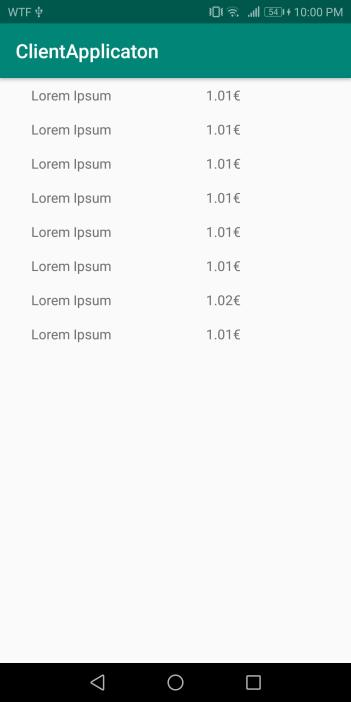
\includegraphics[width=0.35\linewidth]{Images/ProductList.jpg}
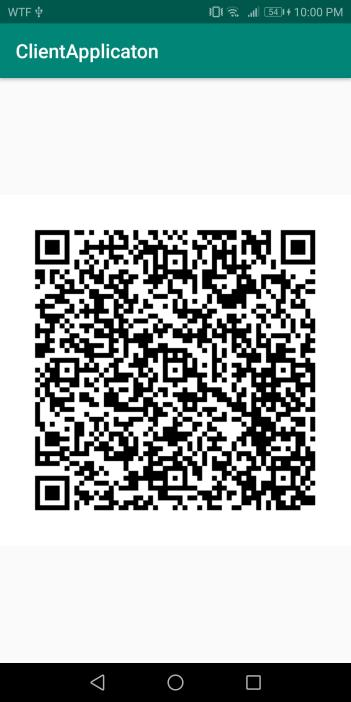
\includegraphics[width=0.35\linewidth]{Images/ProductView.jpg}
\captionof{figure}{Product List and Viewing QR Code From Product In List}
\end{center}

\subsubsection{Checkout}
\hspace{0.6cm}
To perform the client checkout we need to click the "Customer Checkout" button in the store main menu, the camera
will then open up and allow us to scan the QR code, once that is done the purchase will be sent to the server and
processed.

\begin{center}
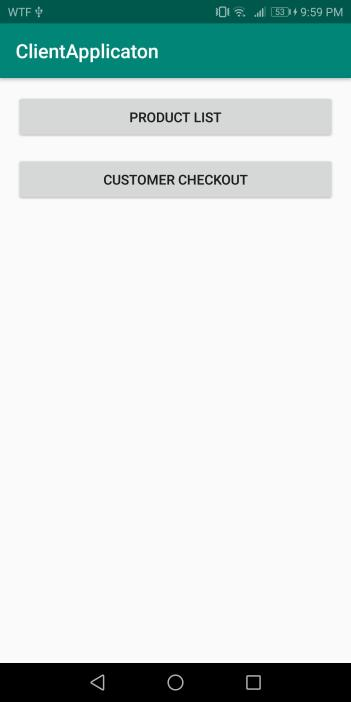
\includegraphics[width=0.35\linewidth]{Images/StoreMenu.jpg}
\captionof{figure}{Store Main Menu}
\end{center}

\subsection{Client Application}

\subsubsection{User Registering}
\hspace{0.6cm}
The user can register in the system by clicking the Register Button in the client app authentication menu, he will
then be taken to the register view, where he will be able to input his data and once registered in the server will
be redirected to the client app main menu.

\begin{center}
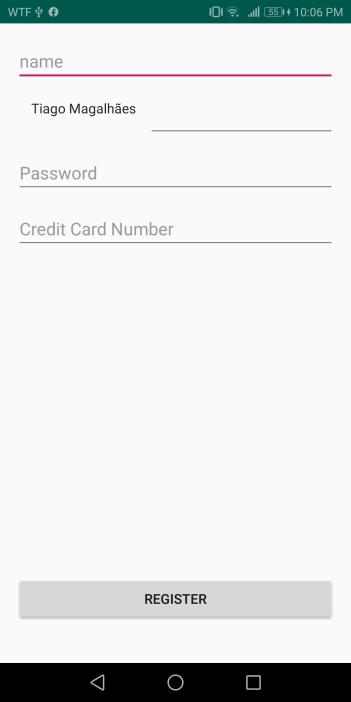
\includegraphics[width=0.35\linewidth]{Images/Client/ClientRegister.jpg}
\captionof{figure}{Register Page}
\end{center}

\subsubsection{User Login}
\hspace{0.6cm}
If a user has logged out of the system but want to log back in he can click the login button in the client app
authentication menu, he will be taken to the login page where he can input his username and password, if that
matches the application credential database he will be taken to the client application main menu

\begin{center}
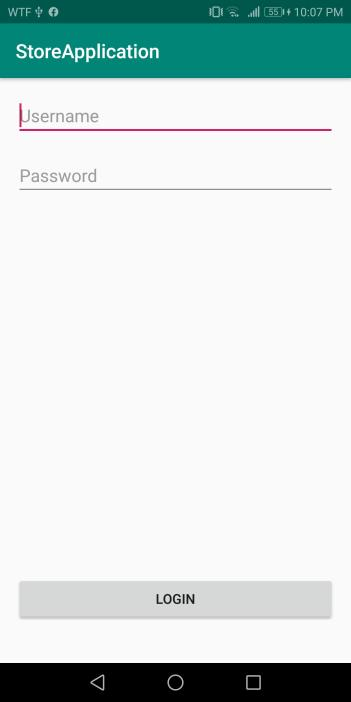
\includegraphics[width=0.35\linewidth]{Images/Client/ClientLogin.jpg}
\captionof{figure}{Login Page}
\end{center}

\subsubsection{User Login Caching}
\hspace{0.6cm}
If the user is currently signed in on the client application, when the application open it will verify this and
if the user is logged in he will be instantly redirected to the client application main menu without having to
to through the manual login process.

\begin{center}
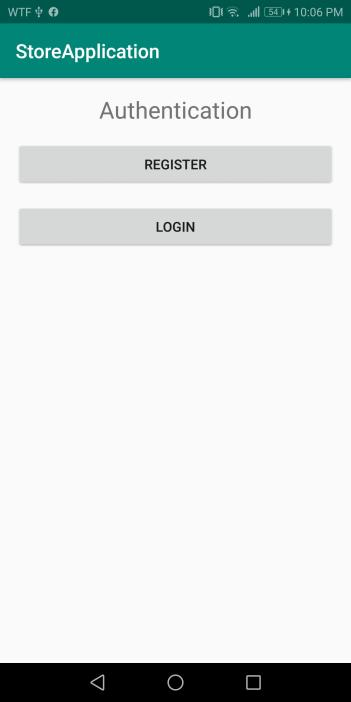
\includegraphics[width=0.35\linewidth]{Images/Client/ClientAuthMenu.jpg}
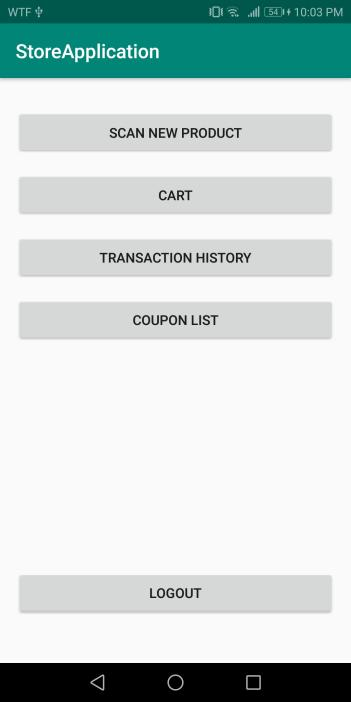
\includegraphics[width=0.35\linewidth]{Images/Client/ClientMainMenu.jpg}
\captionof{figure}{User Login Caching Flow}
\end{center}

\subsubsection{Adding Products To Cart Through QR Codes}
\hspace{0.6cm}
To add a product to the cart the user merely needs to click the scan new product option in the client application
main menu, the camera will then open up and allow the user to scan a new product into the cart. 

\begin{center}
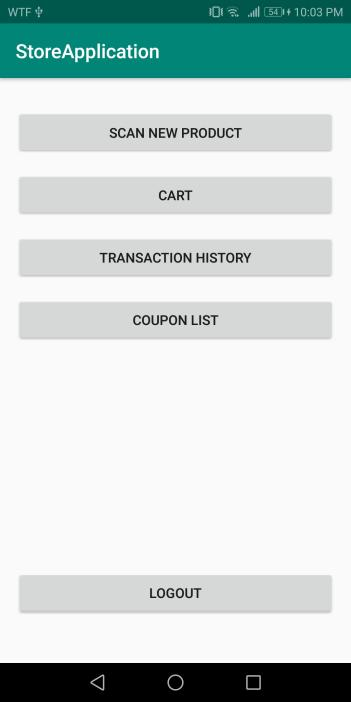
\includegraphics[width=0.35\linewidth]{Images/Client/ClientMainMenu.jpg}
\captionof{figure}{Client Application Main Menu}
\end{center}

\subsubsection{Viewing and Editing Cart}
\hspace{0.6cm}
The user can view his cart by clicking the Cart button in the client application main menu, he will then be taken to a page with
his cart, a list of the products in it and the current price of all those products put together, on any of those products, he can click
the remove button to remove them from the cart.

\begin{center}
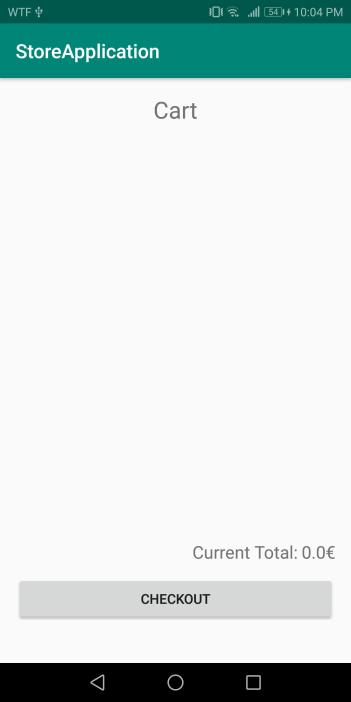
\includegraphics[width=0.35\linewidth]{Images/Client/ClientEmptyCart.jpg}
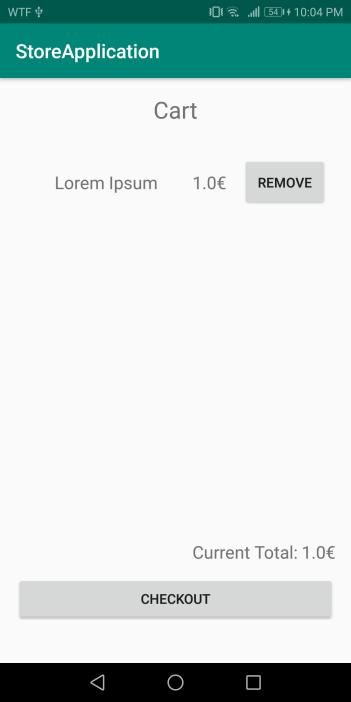
\includegraphics[width=0.35\linewidth]{Images/Client/ClientCart.jpg}
\captionof{figure}{Client Application Main Menu}
\end{center}

\subsubsection{Viewing Past Transaction}
\hspace{0.6cm}
At any time the user can view his past transactions by click the Transaction history button, then he will be taken to a page with a list
of all the transactions he has made in the system.

\begin{center}
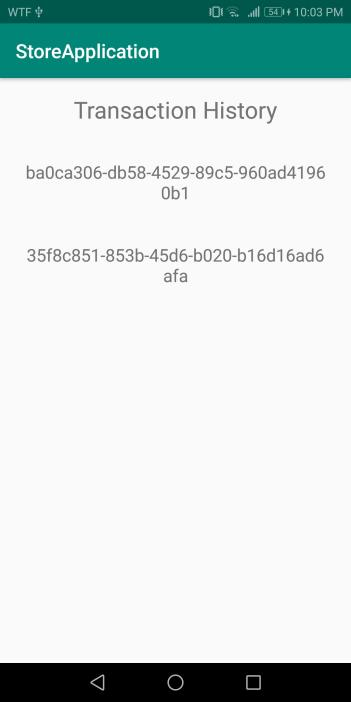
\includegraphics[width=0.35\linewidth]{Images/Client/ClientTransactionHistory.jpg}
\captionof{figure}{Client Transaction History}
\end{center}

\subsubsection{Viewing Products Bough In Past Transaction}
\hspace{0.6cm}
If the user clicks an item in the transaction history list, he will get a list of all the items he purchased in that transaction.

\begin{center}
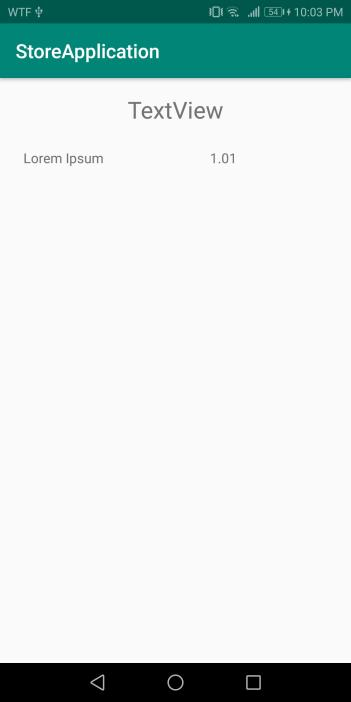
\includegraphics[width=0.35\linewidth]{Images/Client/ClientTransaction.jpg}
\captionof{figure}{Products Bought In Purchase}
\end{center}

\subsubsection{Viewing Vouchers Available To User And Amount Of Money Usable For Discounting}
\hspace{0.6cm}
The user can at any time view the vouches he has available for use by clicking the Coupons button, he will then be taken to a page
with a list of all the coupons he has left to use.

\begin{center}
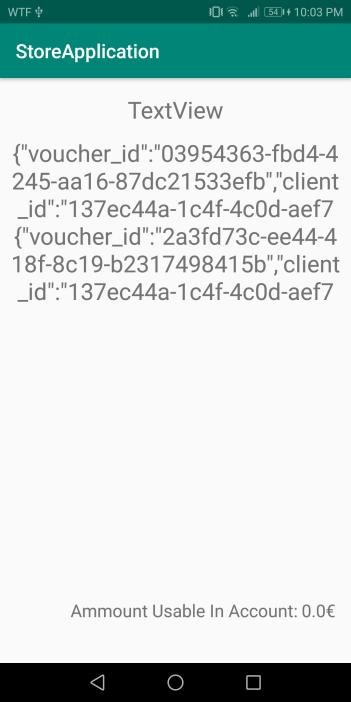
\includegraphics[width=0.35\linewidth]{Images/Client/ClientVoucherList.jpg}
\captionof{figure}{Client Available Voucher List}
\end{center}

\subsubsection{Checkout}
\hspace{0.6cm}
To checkout the user needs to go into his cart and click the checkout button at which point he will be taken to the checkout page where he
can configure the purchase and generate a QR code that he must present to the store app in order to execute the purchase.

\begin{center}
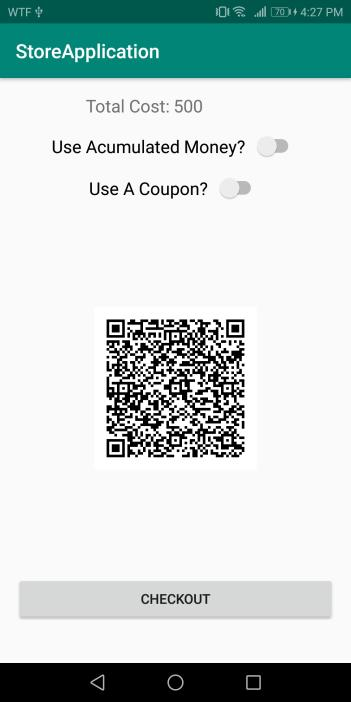
\includegraphics[width=0.35\linewidth]{Images/Client/ClientCheckout.jpg}
\captionof{figure}{Checkout View}
\end{center}

\end{document}
